In this chapter we will consider a one-dimensional optical cavity consisting of two mirrors separated apart by length $L$, the gap will be vacuum. This setup is know as a Fabry-Perot cavity (Cite Laser book). We will allow for a small perturbation to the cavity length $b(t)$, i.e. a movable end mirror, and arriving at the canonical optomechanical model, modeling a cavity with a micro-mirror suspended on a spring (Cite Braginsky or other). The cavity is driven by an input electric field from the left onto the input mirror. We are interested in the magnitude of the circulating intra-cavity electrical field, i.e. the circulation optical power. First we will first quickly sketch the steady-state solution of the field amplitudes (Cite Hecht, Zwickl and bachelor), then depart from the steady-state picture, by allowing the amplitude of all fields to vary on timescale $\sim 2\pi/\omega_{m,n}$, this is much slower than the optical cycle and cavity round trip time $\tau_{rt} = 2L/c$. This treatment will show us the behaviour of slow buildup and decay of the intra-cavity field (Cite Zwickl and\parencite{Wilson2011}).

The transmission line model is sketched in figure \ref{fig:cavity_model}. Consider $E_{in}e^{i\omega_0 t}$, $E_{ref}e^{i\omega_0 t}$ and $E_{out}e^{i\omega_0 t}$ to be complex amplitudes of input, reflected and output traveling waves. What's left is the circulating intra-cavity field of special interest, the total field $E_{circ}e^{i\omega_0 t}$ is given by a superposition of the rigth propagating plane wave $E_{circ}^+e^{i(\omega_0 t + kz)}$ and the left $E_{circ}^-e^{i(\omega_0 t - kz)}$. We can easily write $E_{circ}^-e^{i(\omega_0 t - kz)} = r_2E_{circ}^+e^{i(\omega_0 t + kz)}$. It should be noted that the actual electric field is given as $\Re(E(z, t))$ and that $E(t) \propto e^{-i\omega t}$ corresponds to the Fourier frequency component $E(\omega)$. We will assume flat loss-less mirrors with real reflection coefficients $r_{1,2}$, $t_{1,2}$ and $r_{1,2}^2 + t_{1,2}^2 = 1$, uniform plane waves and a monochromatic carrier of frequency $\omega_0$. The common polarization will be perpendicular to the z-axis. We will call $z = 0$ at the inner surface of the left mirror.

\begin{figure}[h!]
\centering
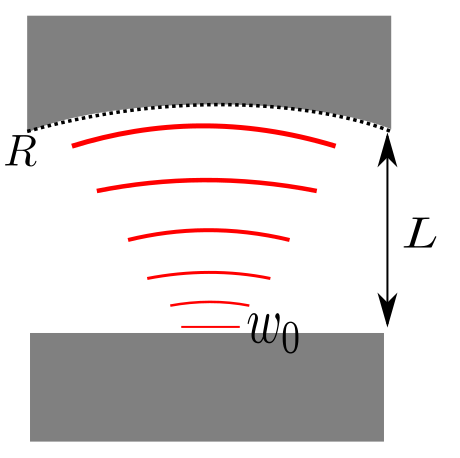
\includegraphics[scale=0.8]{cavity.png}
\caption{Scheme of the one-dimensional optomechanical system.}
\label{fig:cavity_model}
\end{figure}

For the steady-state picture we will be using a mirror transfer matrix, keeping in mind that it has to be unitary.

\begin{equation}
M_{1,2} = 
\begin{pmatrix}
t_{1,2} & -r_{1,2} \\
r_{1,2} & t_{1,2}
\end{pmatrix}
\end{equation}

We can easily write up the transfer matrix of the amplitudes, leaving out $e^{i\omega_0 t}$ since it will drop out

\begin{subequations}
\begin{align}
\begin{pmatrix}
E_{circ}^{+}(z = 0) \\
E_{ref}(z = 0)
\end{pmatrix}
 & = M_{1}
\begin{pmatrix}
E_{in}(z = 0) \\
E_{circ}^{-}(z = 0)
\end{pmatrix} \\
\begin{pmatrix}
E_{trans}^{+}(z = L) \\
E_{c}^{-}(z = L)
\end{pmatrix}
 & = M_{2}
\begin{pmatrix}
E_{circ}^{+}(z = L) \\
0
\end{pmatrix}
\end{align}
\end{subequations}

As a small side remark we could introduce an extra drive field from right by replacing it with the 0 in the equation above, but we will leave it out. If we solve for $E_{circ}^{+}$ and $E_{circ}^{-}$ in terms of $E_{in}$, take the high-reflecting limit $r_{1,2} \rightarrow 1$, introduce the small perturbation $\tilde{L} = L + b$ and $\tilde{k} = k + \delta k$ and define the resonant cavity so that $e^{ikL} = 1$, the intra-cavity fields amplitude becomes equal

\begin{equation}
E_{circ}^{-} = E_{circ}^{+} \equiv E_{cav} \approx t_1 E_{in} \frac{1}{1 - \left|r_1r_2\right|e^{2i(kb + L\delta k)}}
\end{equation}

We have omitted second order terms. This is the textbook steady-state solution of the Fabry-Perot cavity, except for the included small perturbation.